\documentclass[8pt, a4paper, twoside, twoclumn, english]{extreport}
\usepackage{lipsum, babel}
\usepackage{listing}
\usepackage{graphicx}
\graphicspath{ {./images/} }

\begin{document}

\title{CSCI 415 Assignment 2}
\author{Holland Schutte}
\maketitle

\section{Machine Description}

\paragraph{
  The machine specs these benchmarks were ran on feature a 2 numa node architecture,
  complete with 6 cores per node and 2 processing units per core. L3 cache is shared
  across cores, at 15 MB. The L2 and L1 caches are separate for each core, with L2
  at 256kb in size. L1 is comprised of two separate caches,
  one for instructions and one for data. Both of these are 32kb in size each.
}

\section {Results}

\begin{figure}[h]
\caption{}
\centering
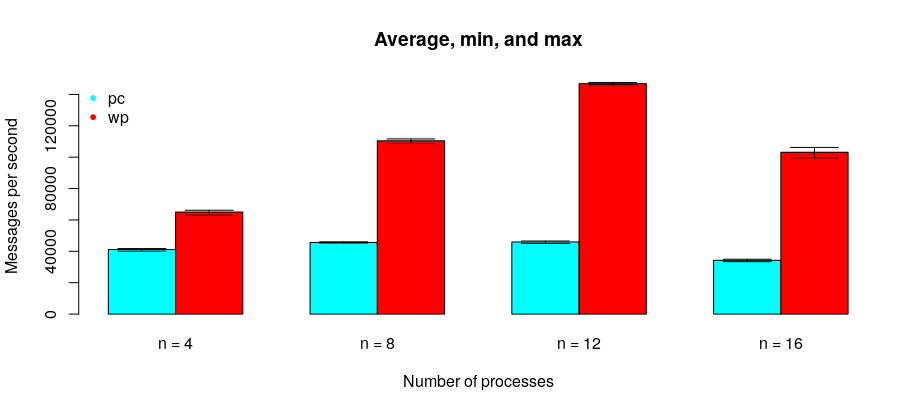
\includegraphics[scale=0.5, height=3.5cm]{avgminmax}
\end{figure}

\subsection {Thoughts}

\paragraph {
  Overall, the model with the most average throughput appears to be the workpool.
  Socket connections can naturally be cached, so it's reasonable to assume that
  the lack of consistency in process 2 process communication buffers doesn't
  really offer any real overhead. On a macro scale, we're multiplying the amount of
  consume counters by 2 (wrt to the producer consumer model),
  and there isn't a need for a strict ordering (at the application level)
  in terms of what is processed and when. The broker model has a component
  that utilizes serialization more so than the workpool model. Each work pool only sends data
  after it's received an ack from a different process as well, so during the
  non-ack period it can continue consuming work from other processes, and thus
  increment the counter at a more frequent rate until that ack is finally received.
  It's a minor aspect that shines best when a significant amount processes
  are all sending to the same destination, but it does contribute a role
  especially since the random seed that's used (at the microsecond level)
  has a reasonable chance of being a similar value across processes.
}

\subsection{Figures}

\begin{enumerate}
\item Producer, consumer
  \begin{itemize}
  \item n = 4; average = 44146, max = 41754, min = 40082
  \item n = 8; average = 45606, max = 46031, min = 45331
  \item n = 12; average = 45964, max = 46544, min = 44972
  \item n = 16; average = 34281, max = 34952, min = 33444
  \end{itemize}
\item Workpool
  \begin{itemize}
  \item n = 4; average = 65048, max = 66170, min = 62996
  \item n = 8; average = 110444, max = 111615, min = 108674
  \item n = 12; average = 146851, max = 147636, min = 146143
  \item n = 16; average = 103162, max = 106228, min = 99607
  \end{itemize}
\end{enumerate}



\end{document}
